\section{Novelty}
\label{sec:novelty}

\Cref{ch:novelty_open_world} developed novelty as an agent-relative mismatch between the world and an agent's knowledge.
Here we formalize that idea within the agent--environment framework of the preceding sections and introduce the taxonomies used throughout the dissertation.

\subsection{An Agent-Relative Definition of Novelty}
\label{sec:novelty_definition}

We depart from treatments that define novelty as an intrinsic property of objects or events \citep{boult2021towards}, and instead adopt an agent-relative view: an aspect of the environment is novel for an agent if and only if the agent cannot represent or derive it from its current knowledge \citep{goel2024neurosymbolic,muhammad2021novelty}.

\begin{definition}[Novelty]
\label{def:novelty}
Let $\Agent$ be an agent with knowledge repository $\KnowledgeRepo = (\KB, \SubsymbolicKB)$ and inference mechanism $\vdash$. A representation $\nu$ of an aspect of an environment state $e \in \EnvStates$ is a \emph{novelty} for $\Agent$ if $\KnowledgeRepo \nvdash \nu$, where $\nu$ may be a symbolic expression in $\Language$ or a subsymbolic representation.
\end{definition}

This definition captures the intuition that novelty is epistemic: what is novel for one agent may be entirely familiar to another. A mass spectrometer is novel to a patient who has never encountered one, but not to the clinician who uses it daily. In the context of task-performing agents, novelty arises whenever the environment presents aspects that fall outside the agent's current representational and inferential capacity.

\Cref{def:novelty} encompasses several distinct ways in which mismatch can manifest. Novelty may involve entirely new elements---objects, predicates, actions, or states that the agent's models do not contain---or it may involve changes in how existing elements behave. Using the planning and learning vocabulary from \cref{sec:agent_framework}, a novelty can induce extensions or modifications of the agent's models such that at least one of the following holds:
\begin{align}
\label{eq:novelty_conditions}
\Fluents' \setminus \Fluents \neq \emptyset, \quad
\Operators' \setminus \Operators \neq \emptyset, \quad
\States' \not\subseteq \States, \quad
\Actions' \not\subseteq \Actions, \quad
\Transition' \neq \Transition.
\end{align}
The first four conditions capture the introduction of entirely new elements that the agent's models do not contain. The fifth condition captures changes in the environment's dynamics for existing state-action pairs---situations where the agent's learned transition model no longer predicts the environment's behavior correctly. This distinction matters because many real-world novelties do not introduce new elements but instead alter how existing elements behave.

\subsection{A Taxonomy of Novelty by Task Impact}
\label{sec:novelty_taxonomy}

In order to reason about how agents should respond to novelty, it is useful to classify novelties by their impact on the agent's ability to achieve its goals. Some novelties may entirely prevent the agent from solving a task, while others may only cause minor disruptions or even present new opportunities for improved performance. To capture this variation, we introduce a taxonomy of novelty types based on how they affect the agent's ability to solve a given planning task $\PlanningTask$.

The following definitions formalize four categories of novelty based on their relationship to the agent's task performance \citep{goel2024neurosymbolic}. In each case, the novelty type is defined relative to a specific agent $\Agent$ and task $\PlanningTask$, since the same environmental change may have different implications for different agents or tasks.

\begin{definition}[Prohibitive Novelty]
\label{def:prohibitive}
A novelty $\nu$ is \emph{prohibitive} for agent $\Agent$ and task $\PlanningTask$ if, for all plans $\Plan$ that $\Agent$ can generate from its current knowledge, $\Plan$ does not solve $\PlanningTask$, but there exists a plan $\Plan_\nu$ that solves $\PlanningTask$ and can be derived from $\KB \cup \{\nu\}$.
\end{definition}

Prohibitive novelties represent aspects of the environment that the agent \emph{must} represent and reason with in order to generate a successful plan. Without accommodating the novelty, no plan exists within the agent's current knowledge that achieves the goal.
For example, in the running example, the agent relies on a crafting table to combine resources into the target item. If no crafting table is available in the current state description, then the agent's existing knowledge contains no valid plan for crafting the pogostick. This constitutes a prohibitive novelty when the environment nevertheless contains an unmodeled way to make the task solvable---for instance, a supplier that can provide a crafting table, a storage container that contains one, or a new recipe that no longer requires one. Until such information is discovered and incorporated into the agent's knowledge base, the agent cannot construct a successful plan.

\begin{definition}[Obstructive Novelty]
\label{def:obstructive}
A novelty $\nu$ is \emph{obstructive} for agent $\Agent$ and task $\PlanningTask$ if it causes the executor $e(\Operator)$ for some operator $\Operator$ in a plan for $\PlanningTask$ to fail---that is, execution completes without $\Abstraction(s') \models \Eff_{\Operator}$ for the post-execution state $s'$.
\end{definition}

Obstructive novelties manifest during plan execution: the agent may construct a symbolic plan that is valid according to its current models, but an operator fails when executed in the environment. For example, in the crafting domain, the agent may plan to break a tree to obtain logs, assuming that trees can be broken directly. If trees now require the agent to hold a tool before they can be broken, the \texttt{break\_tree} operator fails despite being applicable under the agent's prior model, making the novelty obstructive.

\begin{definition}[Beneficial Novelty]
\label{def:beneficial}
A novelty $\nu$ is \emph{beneficial} for agent $\Agent$ and task $\PlanningTask$ if at least one plan derivable from $\KB$ already solves $\PlanningTask$, and there exists a plan $\Plan_\nu$ derivable from $\KB \cup \{\nu\}$ such that $\Plan_\nu$ solves $\PlanningTask$ with lower cost than any plan derivable from $\KB$ alone that also solves $\PlanningTask$.
\end{definition}

When all operators have unit cost, lower cost corresponds to shorter plan length. Beneficial novelties provide new capabilities, resources, or interactions that improve task performance without being necessary for task success. For example, a new tool that accelerates resource collection, or a newly introduced supplier who can provide an ingredient more directly than the agent's existing strategy, would constitute a beneficial novelty. The agent need not accommodate such novelties in order to complete the task, but recognizing them allows it to generate lower-cost plans.

\begin{definition}[Nuisance Novelty]
\label{def:nuisance}
A novelty $\nu$ is a \emph{nuisance} for agent $\Agent$ and task $\PlanningTask$ if at least one plan derivable from $\KB$ already solves $\PlanningTask$, and incorporating $\nu$ into the agent's knowledge does not enable any plan that is shorter or less costly than the best plan derivable from $\KB$ alone.
\end{definition}

Nuisance novelties are aspects of the environment that are genuinely unknown to the agent but have no bearing on task performance. They may cause minor diversions or require brief investigation, but accommodating them yields no task benefit. A new decorative object in the environment, or a change to the visual appearance of an irrelevant entity, would typically constitute nuisance novelties.

These four categories characterize novelties in terms of their impact on the agent's ability to solve a task. A novelty may make planning impossible without additional knowledge (prohibitive), cause failure during plan execution (obstructive), enable a lower-cost plan (beneficial), or fail to improve task performance while also not preventing task completion (nuisance). These categories are agent- and task-relative rather than solely intrinsic properties of the environment: the same environmental change may have different effects for different agents, tasks, or plans. They therefore provide a principled vocabulary for reasoning about what an agent must do in response to a detected novelty.

\subsection{Novelty by Domain Element}
\label{sec:novelty_domain_element}

Orthogonal to the task-impact taxonomy, novelties can also be classified by the type of domain element they affect. Whereas the task-impact taxonomy characterizes how a novelty affects the agent's ability to complete a task, the domain-element taxonomy characterizes what aspect of the environment or agent--environment interaction has changed. Following the NovelGridworlds taxonomy \citep{balloch2022novgrid}, we distinguish three broad classes: object, attribute, and action novelty. This classification is still relative to a particular agent and task, rather than being an intrinsic property of the environment alone.

\paragraph{Object novelty.} Object novelties occur when a previously unknown object or entity appears in the environment. Such an object does not correspond to any category in the agent's current model of the world and may introduce unfamiliar properties, affordances, or constraints. For example, a new fence object may appear around task-relevant resources, requiring the agent to discover how to interact with it before those resources can be accessed.

\paragraph{Attribute novelty.} Attribute novelties occur when a known object remains recognizable, but one or more of its properties or effects changes. In this case, the agent can identify the object, but its prior model of how the object behaves is no longer accurate. For example, breaking a tree may produce a different quantity of wood than expected, or a wall may acquire a dangerous property, such as a fire hazard that penalizes the agent for moving near it.

\paragraph{Action novelty.} Action novelties occur when the agent's action space changes, or when the effects of known actions differ from the agent's expectations. A new action may become available, such as a jump or chop action, or an existing action may be remapped so that it produces a different outcome than before; for example, a move-forward action may unexpectedly move the agent backward. In such cases, the agent must revise its model of what actions are available and what effects they produce.

These two classification schemes---by task impact and by domain element---are complementary. A given novelty can be described both in terms of what changed in the domain and in terms of how that change affects the agent's task performance. For example, a fence is an object novelty because it introduces a new object into the environment, but it may be prohibitive, obstructive, or merely a nuisance depending on whether it blocks access to task-relevant resources and whether the agent has another way to reach them. Similarly, a new chop action is an action novelty, but it may be beneficial if it allows the agent to collect resources more efficiently. \Cref{fig:novelty_taxonomy} illustrates this two-dimensional classification with examples from the crafting scenario introduced in \cref{sec:running_example}.

% Novelty taxonomy figure
\begin{figure}[t]
    \centering
    \resizebox{\textwidth}{!}{%
    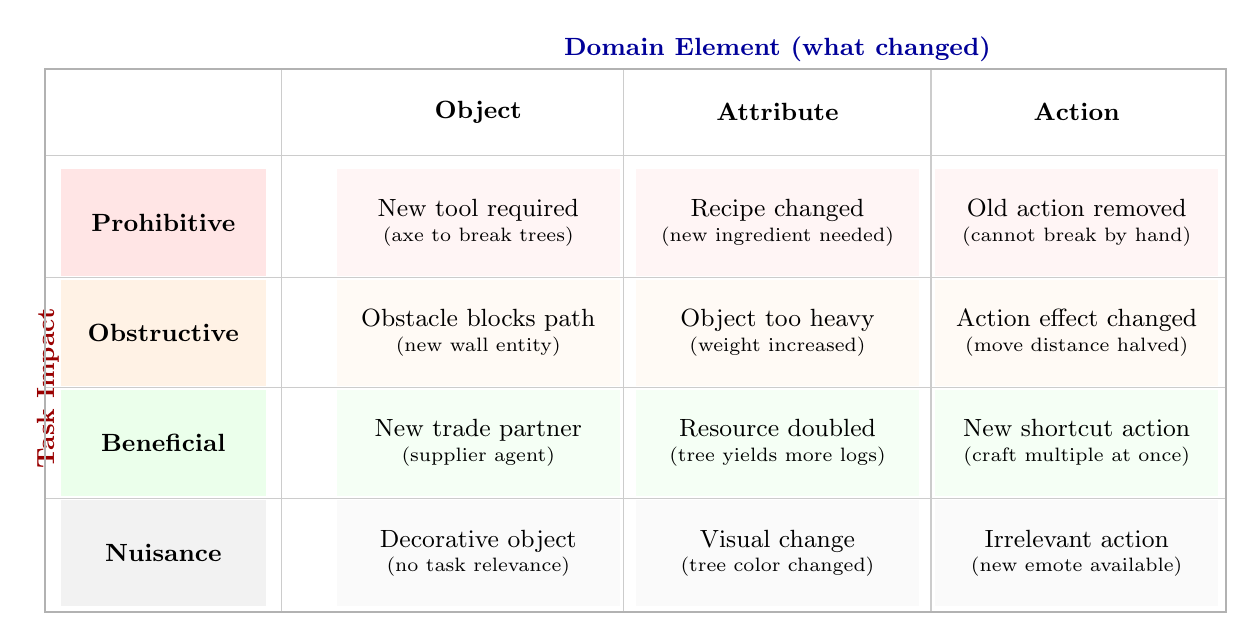
\begin{tikzpicture}[
        % --- Cell styles ---
        cell/.style={
            minimum width=3.6cm, minimum height=1.35cm, 
            align=center, font=\small, inner sep=4pt
        },
        header/.style={
            minimum width=3.6cm, minimum height=0.8cm, 
            align=center, font=\small\bfseries
        },
        rowhead/.style={
            minimum width=2.6cm, minimum height=1.35cm, 
            align=center, font=\small\bfseries
        },
        axislabel/.style={font=\small\bfseries},
    ]

    % ===== Column positions =====
    %  Row headers: x = 0
    %  Col 1 (Object):    x = 4.0
    %  Col 2 (Attribute):  x = 7.8
    %  Col 3 (Action):     x = 11.6

    % ===== Row positions =====
    %  Col headers: y = 0
    %  Row 1 (Prohibitive):  y = -1.4
    %  Row 2 (Obstructive):  y = -2.8
    %  Row 3 (Beneficial):   y = -4.2
    %  Row 4 (Nuisance):     y = -5.6

    % ===== Axis labels =====
    \node[axislabel, text=blue!60!black] at (7.8, 0.8) {Domain Element (what changed)};
    \node[axislabel, text=red!60!black, rotate=90, anchor=south] at (-1.2, -3.5) {Task Impact};

    % ===== Column headers =====
    \node[header] at (4.0, 0.0)  {Object};
    \node[header] at (7.8, 0.0)  {Attribute};
    \node[header] at (11.6, 0.0) {Action};

    % ===== Row headers =====
    \node[rowhead, fill=red!10]    at (0.0, -1.4) {Prohibitive};
    \node[rowhead, fill=orange!10] at (0.0, -2.8) {Obstructive};
    \node[rowhead, fill=green!8]   at (0.0, -4.2) {Beneficial};
    \node[rowhead, fill=gray!10]   at (0.0, -5.6) {Nuisance};

    % ===== Grid lines =====
    % Vertical
    \draw[black!20] (1.5, 0.55) -- (1.5, -6.35);
    \draw[black!20] (5.85, 0.55) -- (5.85, -6.35);
    \draw[black!20] (9.75, 0.55) -- (9.75, -6.35);

    % Horizontal
    \draw[black!20] (-1.5, -0.55) -- (13.5, -0.55);
    \draw[black!20] (-1.5, -2.1) -- (13.5, -2.1);
    \draw[black!20] (-1.5, -3.5) -- (13.5, -3.5);
    \draw[black!20] (-1.5, -4.9) -- (13.5, -4.9);
    \draw[black!20] (-1.5, -6.35) -- (13.5, -6.35);

    % Outer frame
    \draw[black!30, thick] (-1.5, 0.55) rectangle (13.5, -6.35);

    % ===== Prohibitive row =====
    \node[cell, fill=red!4] at (4.0, -1.4)  {New tool required\\[-2pt]{\scriptsize (axe to break trees)}};
    \node[cell, fill=red!4] at (7.8, -1.4)  {Recipe changed\\[-2pt]{\scriptsize (new ingredient needed)}};
    \node[cell, fill=red!4] at (11.6, -1.4) {Old action removed\\[-2pt]{\scriptsize (cannot break by hand)}};

    % ===== Obstructive row =====
    \node[cell, fill=orange!4] at (4.0, -2.8)  {Obstacle blocks path\\[-2pt]{\scriptsize (new wall entity)}};
    \node[cell, fill=orange!4] at (7.8, -2.8)  {Object too heavy\\[-2pt]{\scriptsize (weight increased)}};
    \node[cell, fill=orange!4] at (11.6, -2.8) {Action effect changed\\[-2pt]{\scriptsize (move distance halved)}};

    % ===== Beneficial row =====
    \node[cell, fill=green!4] at (4.0, -4.2)  {New trade partner\\[-2pt]{\scriptsize (supplier agent)}};
    \node[cell, fill=green!4] at (7.8, -4.2)  {Resource doubled\\[-2pt]{\scriptsize (tree yields more logs)}};
    \node[cell, fill=green!4] at (11.6, -4.2) {New shortcut action\\[-2pt]{\scriptsize (craft multiple at once)}};

    % ===== Nuisance row =====
    \node[cell, fill=gray!4] at (4.0, -5.6)  {Decorative object\\[-2pt]{\scriptsize (no task relevance)}};
    \node[cell, fill=gray!4] at (7.8, -5.6)  {Visual change\\[-2pt]{\scriptsize (tree color changed)}};
    \node[cell, fill=gray!4] at (11.6, -5.6) {Irrelevant action\\[-2pt]{\scriptsize (new emote available)}};

    \end{tikzpicture}
    }%
    \caption[Two-dimensional novelty taxonomy]{The two-dimensional novelty taxonomy. Columns classify novelties by the type of domain element affected (object, attribute, or action). Rows classify novelties by their impact on the agent's task performance (prohibitive, obstructive, beneficial, or nuisance). Each cell illustrates the combination with a concrete example from the crafting scenario. Both dimensions are agent-relative: the same environmental change may fall into different categories for different agents depending on their knowledge and current task.}
    \label{fig:novelty_taxonomy}
\end{figure}

Returning to the running example, the axe novelty illustrates how a single environmental change can be classified along both dimensions. The introduction of the axe is an object novelty, and the change to tree-breaking dynamics is an action novelty (the \texttt{break\_tree} action no longer succeeds without holding an axe). At the task-impact level, the novelty is obstructive: the agent can still generate a plan that includes \texttt{break\_tree}, but the executor $e(\texttt{break\_tree})$ fails during execution because the environment now requires a tool the agent's prior executor does not use.
If the agent's architecture decomposes behavior into operators and executors, it can detect that the \texttt{break\_tree} executor failed, identify the mismatch between expected and observed effects, and focus its adaptation on acquiring a new executor for this specific operator. If, on the other hand, the agent uses a monolithic representation, the localization of the failure is not clear, with no indication of what went wrong or what must change, and the agent may need to adapt the entire policy to the new environment. This contrast---between structured and unstructured representations---is the central theme of this dissertation.

\subsection{Novelty in Hybrid Systems}
\label{sec:novelty_hybrid}

The IPT formalism makes explicit where novelty can manifest and how it propagates through the agent's decision-making. Because planning and execution are coupled through the detector $\Abstraction$ and the executor mapping $e$, novelty can break the IPT at two distinct points.

At the \emph{planning level}, novelty may render the symbolic model incomplete: new fluents, new operators, or changed preconditions and effects may mean that no valid plan exists within the agent's current model. The IPT is then not plannable. This corresponds to prohibitive novelty (\cref{def:prohibitive}) and requires symbolic model revision---discovering new operators, fluents, or task structure---before execution can proceed.

At the \emph{execution level}, novelty may cause an executor to fail while the symbolic plan remains valid: the environment dynamics have changed such that $e(\Operator)$ no longer achieves $\Eff_{\Operator}$, even though $\Pre_{\Operator}$ is satisfied under $\Abstraction$. The IPT remains plannable but is no longer solvable, yielding the kind of problem later formalized as a stretch-IPT (\cref{def:stretch_ipt}). This corresponds to obstructive novelty (\cref{def:obstructive}) and manifests as a discrepancy between expected and observed symbolic states after an operator is dispatched for execution.

This distinction is operationally significant. Prohibitive novelties demand changes to $\PlanningDomain$ or $\Operators$; obstructive novelties demand changes to the executor mapping $e$---learning or replacing executors for operators whose symbolic specifications remain valid. \Cref{ch:rapid_learn} develops a neurosymbolic architecture that addresses both failure modes through a cascading recovery pipeline, and formalizes obstructive failures as an \emph{executor discovery problem} in which the agent learns new executors for failed operators while preserving the existing symbolic plan structure.

In either case, the hybrid decomposition localizes failure. When an executor fails, the agent knows \emph{which} operator was being executed and can compare $\Eff_{\Operator}$ against $\Abstraction(s')$ for the post-execution state $s'$. This converts what would otherwise be a global performance degradation into a targeted adaptation problem. Without this structure, a failure in the environment would be an undifferentiated signal with no indication of what specifically went wrong.

This observation motivates the central claim of the dissertation: that structured abstractions over actions and interactions determine whether novelty-induced mismatch can be resolved efficiently and whether learned behaviors can generalize across variations. The next section develops this argument formally.
